\paragraph{Sơ đồ tuần tự luồng Pha khởi tạo giao dịch mua gói thuê bao VIP}

Luồng nghiệp vụ này mô tả
bước User chọn gói thuê bao VIP trên Web Frontend, hệ thống kiểm tra gói dịch vụ, chuẩn bị Subscription, tạo Transaction ở trạng thái \texttt{pending}, đăng ký job timeout trên Redis BullMQ, sau đó gọi Payment Gateway để sinh đường link thanh toán.

\begin{figure}[H]
\centering
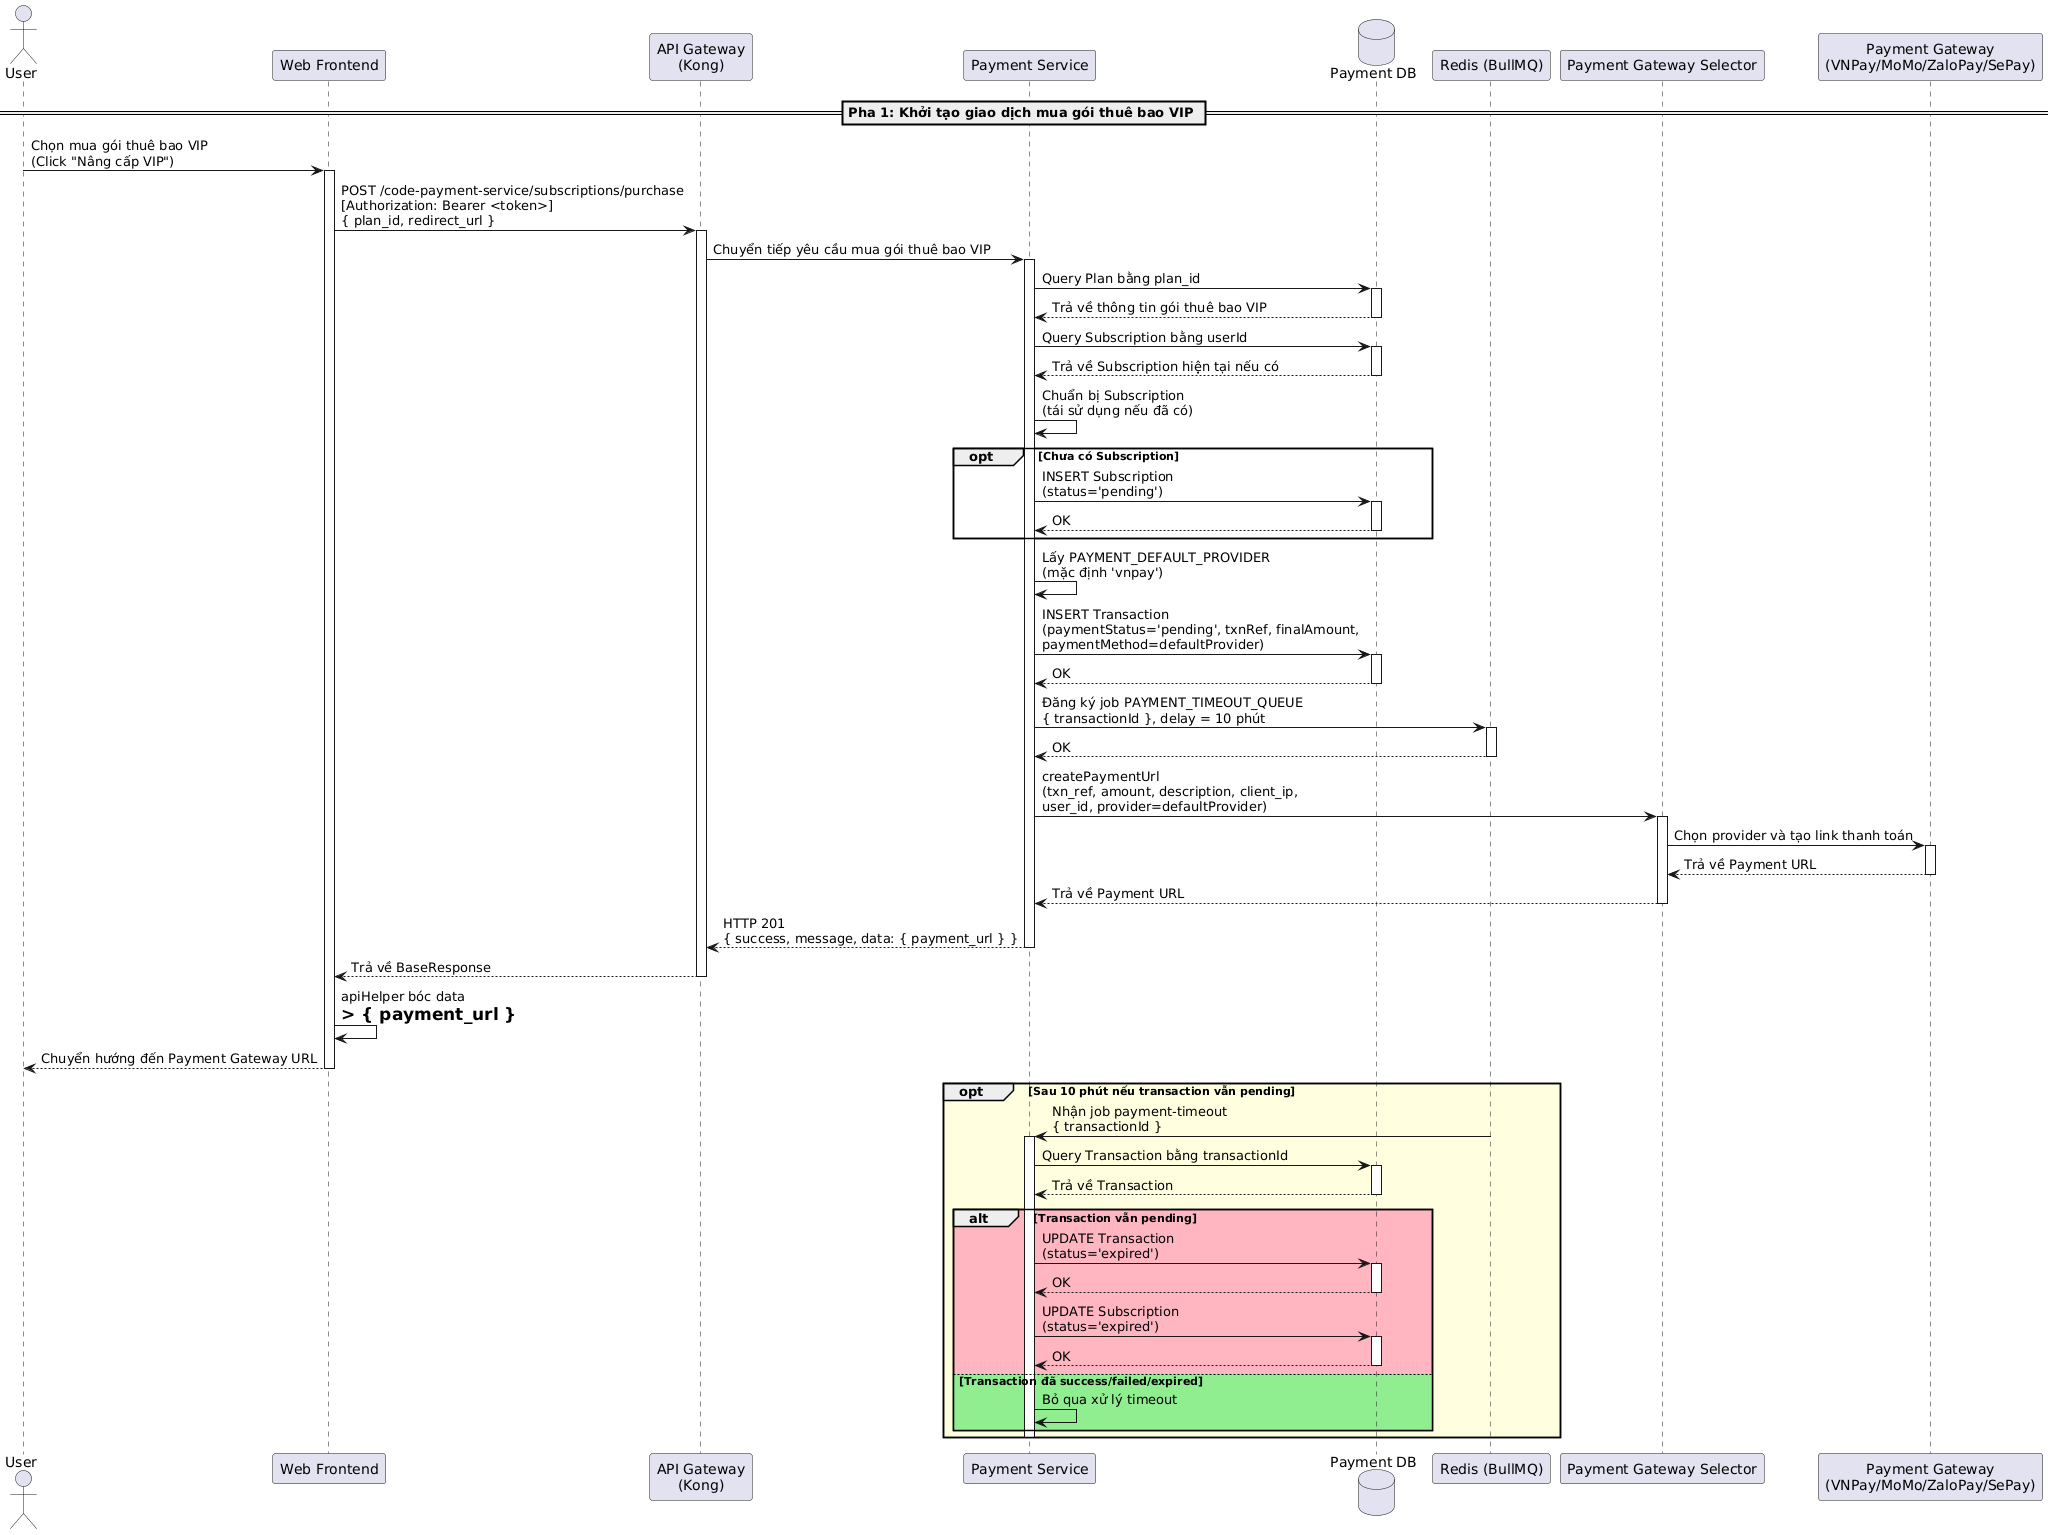
\includegraphics[scale = 0.18]{contents/Sequence/UML-Sequence-UserCreateVipPaymentTransaction.png}
\caption{Sơ đồ tuần tự luồng Pha khởi tạo giao dịch mua gói thuê bao VIP}
\end{figure}

\subparagraph{Các thành phần tham gia}

\begin{table}[H]
\centering
\renewcommand{\arraystretch}{1.3}
\begin{tabular}{|l|l|p{5cm}|}
\hline
\textbf{Thành phần} & \textbf{Phân loại} & \textbf{Vai trò trong hệ thống} \\ \hline
User & Actor & Người dùng đã đăng nhập và chọn mua gói thuê bao VIP. \\ \hline
Web Frontend & Component & Giao diện web Next.js. \\ \hline %%%% Component & Gửi yêu cầu mua gói thuê bao VIP, nhận \texttt{payment\_url} sau khi \texttt{apiHelper} bóc \texttt{data}, rồi chuyển hướng người dùng đến link thanh toán. \\ \hline
API Gateway (Kong) & Component & Cổng API chuyển tiếp các yêu cầu API. \\ \hline %%%% Component & Kiểm tra xác thực token và định tuyến yêu cầu đến Payment Service. \\ \hline
Payment Service & Microservice & Kiểm tra plan, chuẩn bị subscription, tạo transaction, đăng ký timeout job và yêu cầu link thanh toán từ gateway provider mặc định. \\ \hline
Payment DB & Database & Lưu thông tin gói thuê bao VIP, subscription và transaction. \\ \hline
Redis (BullMQ) & Component & Quản lý job \texttt{PAYMENT\_TIMEOUT\_QUEUE} để hết hạn giao dịch sau 10 phút. \\ \hline
Payment Gateway Selector & Component & Chọn cổng thanh toán theo \texttt{PAYMENT\_DEFAULT\_PROVIDER}, mặc định là \texttt{vnpay}. \\ \hline
Payment Gateway & External Service & Cổng thanh toán bên thứ ba sinh Payment URL, hiện có các adapter VNPay, MoMo, ZaloPay và SePay. \\ \hline
\end{tabular}
\caption{Các thành phần tham gia luồng pha khởi tạo giao dịch mua gói thuê bao VIP}
\end{table}

\subparagraph{Mô tả tổng quan}
\begin{itemize}
\item \textbf{Gửi yêu cầu mua gói thuê bao VIP:} User chọn nâng cấp VIP, Frontend gọi \texttt{POST /code-payment-service/subscriptions/purchase} qua Kong kèm Bearer Token và body gồm \texttt{plan\_id}, \texttt{redirect\_url}.
\item \textbf{Chuẩn bị dữ liệu thanh toán:} Payment Service kiểm tra plan còn active, tìm subscription hiện tại của user, tái sử dụng subscription nếu đã có hoặc tạo mới subscription trạng thái \texttt{pending} nếu chưa có.
\item \textbf{Tạo transaction và timeout job:} Service lấy \texttt{PAYMENT\_DEFAULT\_PROVIDER} với mặc định \texttt{vnpay}, tạo transaction mới với \texttt{paymentStatus='pending'}, \texttt{txnRef}, \texttt{finalAmount}, \texttt{paymentMethod}, rồi đăng ký job timeout trên BullMQ với delay 10 phút.
\item \textbf{Tạo link thanh toán:} Service gọi Payment Gateway Selector để chọn provider tương ứng và tạo \texttt{payment\_url}. Backend trả \texttt{BaseResponse} dạng \texttt{\{ success, message, data: \{ payment\_url \} \}}, sau đó Frontend dùng \texttt{apiHelper} bóc \texttt{data} để nhận trực tiếp \texttt{\{ payment\_url \}}.
\item \textbf{Xử lý timeout:} Nếu sau 10 phút transaction vẫn ở trạng thái \texttt{pending}, Payment Timeout Processor cập nhật Transaction và Subscription liên quan thành \texttt{expired}; nếu transaction đã ở trạng thái \texttt{success}, \texttt{failed} hoặc \texttt{expired} thì bỏ qua job timeout.
\end{itemize}
